\documentclass{article}
\usepackage[utf8]{inputenc}
\usepackage{geometry}
\usepackage{graphicx}
\usepackage{pgfplots}
\usepackage{amsmath}
\usepackage{amssymb}
\usepackage{amsfonts}
\usepackage{mdframed}
\usepackage{amsthm}
\usepackage{physics}
\usepackage{derivative}

\geometry{a4paper, left=2cm, right=2cm, top=1cm, bottom=2cm}

\pgfplotsset{compat=1.18}
\begin{document}

\begin{minipage}{0.7\textwidth}
    \small \textbf{LABORATORIO DE MECÁNICA VECTORIAL}  \\
    \small {Facultad de Ciencias, Universidad Nacional Autónoma de México} \\
    \small {Profesor: Radamés Ricardo Reynoso Manríquez} \\
    \small {Ayudante: Ana Laura Córdova Lara}\\
    \small {Fecha de entrega: 02 de Abril de 2024} \\
    \small {Nombre completo: Andrés López González} \\
    \small {Tarea número VI}
\end{minipage}
\hfill
\begin{minipage}{0.12\textwidth}
    
\includegraphics[width=\linewidth]{logo_universidad}
\end{minipage}

\section*{Cuestionario IV}

PREGUNTA 1. La figura 1 muestra la trayectoria seguida por un Learjet de la NASA en una carrera diseñada para simular las condiciones de baja gravedad durante un corto periodo de tiempo. Dé un argumento que demuestre que, si el aeroplano sigue una trayectoria parabólica particular, los pasajeros experimentarán la sensación de ingravidez. \\
\begin{figure} [h]
    \centering
    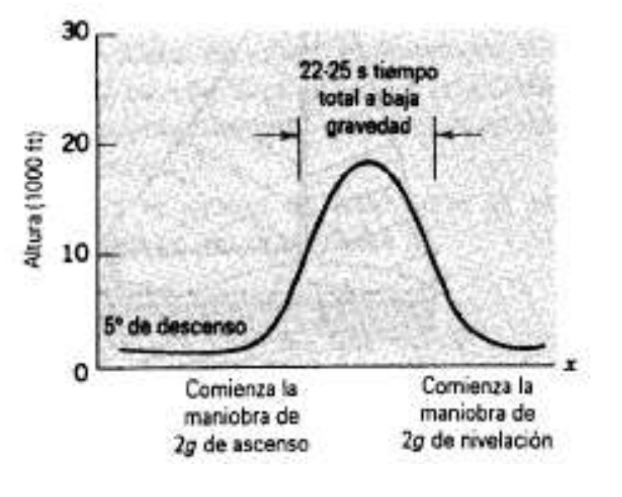
\includegraphics[width=0.5\linewidth]{I.png}
    \caption{Learjet de la NASA}
    \label{fig:enter-label}
\end{figure} \\\\
\textit{El vuelo parabólico es una técnica utilizada desde los 80s para realizar experimentaciones con la ingravidez, en el primer tramo del recorrido el avión comienza a ascender súbitamente, en esta gráfica no se indica pero generalmente es a 50 grados, esta aceleración hacia arriba genera la sensación de 2g lo cual es denomiado hipergravitación, posteriormente está lo interesante, que es lo requerido en este inciso, el avión deja de acelerar por lo que en algún momento llega a su cresta el tiro parabólico y experimenta caída libre en todo este segmento, es aquí donde entra la microgravedad que contiene la ingravidez, el avión acelera en su descenso a $\approx 9.8066 \frac{m}{s}$ lo cual genera la sensación de 0g, pues contraresta las fuerzas del peso y la normal haciendo que se encuentre en un pseudo perfecto equilibro en las fuerzas, este periodo dura aproximadamente 22-25 segundos, si la gravedad es totalmente 0 en algún momento es debatible pero teóricamente sí lo es infinitesimalmente, aún así la sensación alrededor de ese punto es prácticamente de 0g.} \\\\

PREGUNTA 2. Las piezas de artillería de largo alcance no se colocan en el ángulo de “alcance máximo” de 45°, sino en ángulos de elevación más grandes, en el intervalo de 55° a 65°. ¿Qué hay de malo en los 45°? \\
\textit{Debido a multiples factores, un tiro parabólico maximiza su tiempo de vuelo al estar lo más vertical posible, como evidentemente el proyectil no se quiere lanzar a sí mismo la opción más equilibrada es este intervalo pues se acerca a un alcance horizontal máximo al mismo tiempo que su recorrido tarda más, esto se busca dado que al tardar un mayor tiempo la aceleración gravitacional acelerará mucho más al objeto, en respuesta, la tasa de cambio del ímpetu respecto al tiempo será muy fuerte dado que la velocidad estará cambiando muy bruscamente, lo que por defición es una fuerza muy elevada.}
\begin{equation}
\Vec{F} = \dv{\Vec{P}}{t} \, \propto \, \Vec{\dot{v}}
\end{equation}
\\

\newpage
PREGUNTA 3. En la figura 2 se muestran las trayectorias de tres balones pateados. Escoja la trayectoria para la cual (a) el tiempo de vuelo es menor, (b) la componente vertical de la velocidad al patearlo es la más grande, (c) la componente horizontal de la velocidad al patearlo es más grande, y (d) la velocidad de despegue es la menor. Desprecie la resistencia del aire. \\
\begin{figure}[h]
    \centering
    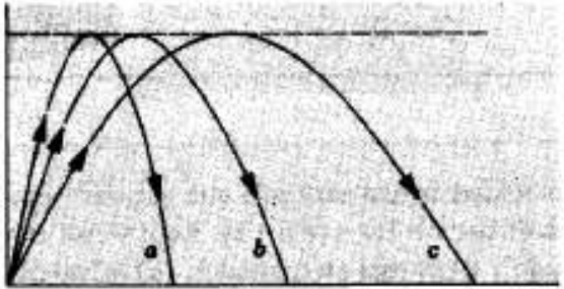
\includegraphics[width=0.5\linewidth]{III.png}
    \caption{Tiros parabólicos.}
    \label{fig:enter-label}
\end{figure} \\
\textit{Todos estos incisos se derivan del experimento del tiro parabólico cuando el objeto en cuestión ha sido desplazado en el eje x con distintas velocidades; para a), observamos el movimiento solo en el eje y, por acción gravitacional y el alcance vertical que tienen (igual) se concluye que estos cuerpos recorren distancias iguales en tiempos iguales pues de no ser así implicaría cambios extraños en las velocidades del sistema y en consecuencia que la aceleración sea distinta a la gravitacional, algo imposible bajo las condiciones planteadas. Con un análisis similar vemos para b) que al recorrer distancias iguales en tiempos iguales al solo observar el eje y por ende la velocidad vertical es la misma siempre, para c) si ya deducimos que el tiempo siempre es el mismo observamos que en una gráfica x vs t el tiro A es el que menos se mueve en un tiempo T, el tiro B se mueve más pero el tiro C recorre la mayor distancia en el mismo tiempo, por lo que su velocidad al considerar distancia/tiempo es la mayor de todas. Finalmente para la velocidad de despegue menor consideramos cual de las velocidades vectoriales su norma es menor, como ya hemos visto que la velocidad en y siempre es igual entonces solo debemos ver que la magnitud de la velocidad en x en algún movimiento debe ser la menor, y es así, como dijimos anteriormente el de menor velocidad horizontal es A por desplazarse menos en el mismo tiempo que todos, por ende este es el de velocidad de despegue menor.} \\\\

PREGUNTA 4. Investiga y explica, el caso real del lanzamiento de un cohete y las diferencias que hay con el modelo de tiro parabólico, respondiendo a las siguientes preguntas: ¿Qué variables están involucradas en el caso real? ¿Qué se entiende (o define) como “restricciones” al sistema? ¿Qué variables se consideran constantes en un movimiento de este tipo? \\
\textit{En mecánica vectorial hemos visto que el lanzamiento real de un cohete es un fenómeno físico muy distinto del modelo simplificado de tiro parabólico. Requiere considerar diversas variables dinámicas y técnicas, como la masa del cohete pues tan solo para la fuerza vemos que la tasa de cambio del ímpetu respecto al tiempo no es solo $m\Vec{a}$ dado que la masa del cohete varía respecto al tiempo (muy importante al atravesar corrientes como el viento), el empuje del motor, la pérdida de energía con el trabajo transferido a calor por el rozamiento del aire que causa fricción cinética, la resistencia aerodinámica, la gravedad terrestre y el ángulo de inclinación. Además, hay restricciones técnicas y físicas a tener en cuenta, como la capacidad de carga, la disponibilidad de propelentes y las condiciones atmosféricas; aunque algunas escasas variables se mantienen constantes, como la gravedad terrestre y la masa del cohete en intervalos infinitesimales, otras varían durante el vuelo.}
\\\\

PREGUNTA 5. Defina y exprese matemáticamente los parámetros de ‘altura máxima’, y de ‘alcance máximo’, en un tiro parabólico? ¿Qué efecto tiene la masa del proyectil \\
\textit{Dadas las 5 ecuaciones fundamentales de la cinemática vectorial podemos derivar de ellas la altura máxima.}
\begin{equation}
h_{\text{max}} = \frac{{v_0^2 \sin^2(\theta)}}{{2g}}
\end{equation}
\textit{Y el alcance horizontal.}
\begin{equation}
R = \frac{{v_0^2 \sin(2\theta)}}{{g}}
\end{equation}
\textit{En donde theta indica evidentemente el ángulo del vector velocidad tangencial respecto al eje ordenado, g la gravedad y $v_0$ la velocidad inicial. Vemos que en ninguna parte es involucrada la fuerza, o alguna magnitud que involucre la masa, por lo cual en un tiro parabólico la masa NO tiene ningún efecto. Claro que en condiciones reales mantener la velocidad tangencial inicial constante a pesar de la masa ya tiene implicaciones con la fuerza pues esta necesita ser más alta en aquel primer instante, pero para efectos del tiro parabólico mientras aseguremos que las demás condiciones se mantienen iguales la masa es indiferente en el tiempo y la trayectoria.} \\
\begin{figure} [h]
    \centering
    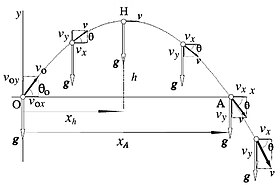
\includegraphics[width=0.3\linewidth]{Cyn.png}
    \caption{Cinemática del tiro parabólico.}
    \label{fig:enter-label}
\end{figure}
\end{document}
